%% This document is created by 
%%  Dr. Putu Harry Gunawan
%% Template untuk Proposal TA 1 dan TA
%% Template ini digunakan untuk penulisan proposal TA 1 atau TA Fakultas Informatika, Telkom University.

\documentclass[a4paper,12pt,oneside]{book}
\usepackage[utf8]{inputenc}
\usepackage{sectsty}
\usepackage{graphicx}
\usepackage{epstopdf}
\usepackage{algorithm}
\usepackage{algpseudocode}
\usepackage{array}
\usepackage[table]{xcolor}
\usepackage{anysize}
\usepackage{amsmath}
\usepackage{amssymb}
\usepackage[bahasa]{babel}
\usepackage{indentfirst} %Spasi untuk paragraf pertama
\usepackage{geometry}
\usepackage{multirow}% http://ctan.org/pkg/multirow
\usepackage{hhline}% http://ctan.org/pkg/hhline
\marginsize{4cm}{3cm}{3cm}{3cm} %{left}{right}{top}{bottom}
\usepackage[compact]{titlesec} 
\usepackage{etoolbox}

\makeatletter
\patchcmd{\ttlh@hang}{\parindent\z@}{\parindent\z@\leavevmode}{}{}
\patchcmd{\ttlh@hang}{\noindent}{}{}{}
\makeatother

\chapterfont{\centering}
\newcommand{\bigsize}{\fontsize{16pt}{14pt}\selectfont}
\chapterfont{\centering\bigsize\bfseries}
\sectionfont{\large\bfseries}
\usepackage{tikz}
\usetikzlibrary{shapes.geometric, arrows}
%\renewcommand{\chaptertitle}{BAB}
\renewcommand{\thechapter}{\Roman{chapter}}
\renewcommand\thesection{\arabic{chapter}.\arabic{section}}
\renewcommand\thesubsection{\thesection.\arabic{subsection}}
\renewcommand{\theequation}{\arabic{chapter}.\arabic{equation}}
\renewcommand{\thefigure}{\arabic{chapter}.\arabic{figure}}
\renewcommand{\thetable}{\arabic{chapter}.\arabic{table}}

\renewcommand\bibname{Daftar Pustaka}
\addto{\captionsbahasa}{\renewcommand{\bibname}{Daftar Pustaka}}
\usepackage{fancyhdr}
\pagestyle{fancy}
\lhead{}
\chead{}
\rhead{}
\lfoot{}
\cfoot{\thepage}
\rfoot{}
\renewcommand{\headrulewidth}{0pt}

\makeatletter

%%%%%%%%%%%%%%%%%%%%%%%%%%%%%%%%%%%%%%%%%%%%%%%%%%%%%%%%%%%%
%
%  Berikut adalah data-data yang wajib diisi oleh mahasiswa
%
%%%%%%%%%%%%%%%%%%%%%%%%%%%%%%%%%%%%%%%%%%%%%%%%%%%%%%%%%%%%

\title{Penerapan Metode Feature Extraction Pada Deteksi Premature Ventricular Contractions (PVCs)}\let\Title\@title   %Judul dalam bahasa Indonesia

\newcommand{\EngTitle}{Implementation Feature Extraction Method in Premature Ventricular Contractions (PVCs) Detection}  %Judul dalam bahasa Inggris

\author{Ihda Husnayain}  \let\Author\@author  %Nama mhs
\newcommand{\NIM}{1103130028}
\newcommand{\Prodi}{Teknik Informatika}
\newcommand{\KK}{Telematics } %UNTUK TA
\newcommand{\Gelar}{komputer} % UNTUK TA
\date{2016}           \let\Date\@date %Maskkan hanya tahun saja
\newcommand{\Tanggal}{7} % Tanggal Pengesahan
\newcommand{\Bulan}{Agustus} % Bulan Pengesahan
\newcommand{\PembimbingSatu}{Satria Mandala, S.T., M.Sc, Ph.D}
\newcommand{\NIPPembimbingSatu}{15731897-3}
\newcommand{\PembimbingDua}{M. Syahrul Mubarok, S.T., M.Sc}
\newcommand{\NIPPembimbingDua}{10830757-3}
\newcommand{\Kaprodi}{Ir. Moch. Arif Bijaksana, M.Tech, Ph.D}
\newcommand{\NIPKaprodi}{03650312-4}
\newif\iflogTA
\logTAtrue   %%%%%% WARNING kode ini diaktifkan untuk format TUGAS AKHIR
\makeatother
\linespread{1}


\begin{document}
\pagenumbering{roman} 
%%\maketitle
\begin{titlepage}
\thispagestyle{empty}
%\vspace*{0.7cm}
{\centering
\large
{\bigsize\bf \Title}\\
\vspace{ 2cm}
\rm
\iflogTA
\textbf{Tugas Akhir}\\
\vspace{0.5 cm}
\textbf{Kelompok Keahlian: Telematika\KK}\\
\else
\textbf{Proposal Tugas Akhir}\\
\vspace{0.5 cm}
\textbf{Kelas TA 1}\\
\fi
\vspace{0.5 cm}
\textbf{\Author}\\ \textbf{NIM: \NIM}\\ 

\vspace{1.5 cm}

\begin{figure}[h]
{\centering {
\includegraphics[scale=0.17]{Tel-U-Logo}}\par}
\end{figure}

\vspace{2 cm}
{\bigsize\textbf{Program Studi Sarjana \Prodi}\\
\vspace{0.5 cm}
\textbf{Fakultas Informatika}\\
\vspace{0.5 cm}
\textbf{Universitas Telkom}\\
\vspace{0.5 cm}
\textbf{Bandung}\\
\vspace{0.5 cm}
\textbf{\Date}\\}
}
\pagebreak
\thispagestyle{empty}
{\centering
\iflogTA
\textbf{\large Lembar Pengesahan}\\  %UNTUK TA
\else
\textbf{\large Lembar Persetujuan}\\
\fi
\vspace{0.5cm}
\textbf{\Title}\\
\vspace{0.5cm}
\textbf{\textit{\EngTitle}}\\
\vspace{0.5cm}
\textbf{\Author}\\
\textbf{NIM: \NIM}\\
\vspace{1cm}

\iflogTA 
{ Tugas Akhir ini diterima dan disahkan untuk memenuhi sebagian dari syarat untuk memperoleh gelar sarjana \Gelar\\ Program Studi Sarjana \Prodi\\ Fakultas Informatika Universitas Telkom}\\  %% UNTUK TA
\else
{ Proposal ini diajukan sebagai usulan pembuatan tugas akhir pada\\ Program Studi Sarjana \Prodi\\ Fakultas Informatika Universitas Telkom}\\
\fi
\vspace{0.5cm}

{Bandung, \Tanggal\quad \Bulan \quad \Date}\\
{Menyetujui}\\

\vspace{0.5cm}
\iflogTA
\begin{center}
\begin{tabular}{  m{8cm}  m{8cm} }
Pembimbing 1 & Pembimbing 2
\end{tabular}
\end{center}
\else
\begin{center}
\begin{tabular}{  m{8cm}  m{8cm} }
Calon Pembimbing 1 & Calon Pembimbing 2
\end{tabular}
\end{center}
\fi
\begin{center}
\vspace{2cm}
\begin{tabular}{  m{8cm}  m{8cm} }
\underline{\PembimbingSatu} & \underline{\PembimbingDua} \\ 
NIP: \NIPPembimbingSatu & NIP: \NIPPembimbingDua
\end{tabular}
\end{center}
\vspace{0.5cm}
\iflogTA
Mengesahkan,\\   %% UNTUK TA
Kepala Program Studi \Prodi\\ %% UNTUK TA
\vspace{2.5cm}   %% UNTUK TA
\underline{\Kaprodi}\\ NIP: \NIPKaprodi\\  %% UNTUK TA
\fi
}
\pagebreak
\end{titlepage}
\addcontentsline{toc}{chapter}{Abstrak}
\chapter*{Abstrak}
%--Overview-- \\
Premature Ventricular Contractions (PVCs) adalah salah satu jenis kelainan jantung yang disebabkan terjadinya kontraksi ventrikel jantung yang tidak biasa, menyebabkan pola denyut jantung menjadi tidak normal atau disebut juga sebagai aritmia dan jika dibiarkan PVC dapat menjadi gejala aritmia lain yang lebih berbahaya. 

Dalam beberapa dekade ini telah banyak diajukan metode untuk melakukan deteksi terjadinya PVC. Pada umumnya metode deteksi ini menganalisa sinyal EKG (Elektrokardiogram) dari pasien. Metode deteksi terdiri dari 4 tahap, yaitu \textit{pre-processing} terhadap sinyal EKG, \textit{feature extraction} dan  \textit{classification}. 
%--Problem-- \\
Nilai akurasi yang diperoleh dari keseluruhan proses deteksi sangat dipengaruhi oleh akurasi bentuk sinyal EKG yang dihasilkan pada tahap \textit{feature extraction}. Oleh karena itu penggunaan algoritma \textit{feature extraction} yang akurat menjadi penting. Dari sekian banyak litaratur yang mengajukan metode deteksi PVC, banyak diantaranya hanya berfokus pada mencari nilai akurasi pada tahap \textit{classification}. Padahal metode \textit{classification} adalah metode yang cukup lama memakan waktu dalam proses. 
%--Objective-- \\
Maka dari itu dalam tugas akhir ini penulis akan melakukan analisis dan pengembangan terhadap algoritma \textit{feature extraction} khusus untuk mendeteksi terjadinya PVC. Dengan adanya algoritma \textit{feature extraction} yang akurat, diharapkan dapat tetap menghasilkan hasil deteksi PVC yang akurat meskipun menggunakan proses \textit{classification} yang sederhana. Sehingga hal ini akan membuat proses deteksi menjadi lebih efisien. 
%--Methodology-- \\
%--Outcome-- \\
Algoritma ekstraksi ciri yang akan digunakan dalam penelitian ini adalah \textit{Windowing Algorithm} yang diusulkan oleh Muhammad Umer(2014) dan algoritma klasifikasi PVC yang diusulkan oleh Ik-Sung Cho(2013). Berdasarkan hasil pengujian dari penerapan algoritma di atas, penelitian ini memperoleh nilai akurasi deteksi sebesar xx\%.
  
\vspace{0.5 cm}
\begin{flushleft}
{\textbf{Kata Kunci:} PVCs, Feature Extraction, Windowing Algorithm.}
\end{flushleft}
\iflogTA
\pagebreak
\addcontentsline{toc}{chapter}{Abstract}
\chapter*{Abstract}

  My abstract here

\vspace{0.5 cm}
\begin{flushleft}
{\textbf{Keywords:} Shallow, water, equations.}
\end{flushleft}
\pagebreak
\addcontentsline{toc}{chapter}{Lembar Persembahan}
\chapter*{Lembar Persembahan}

  Saya persembahkan
  \begin{enumerate}
      \item Kepada Tuhan Yang Maha Esa
      \item Kepada Kedua Orangtua saya
      \item Kepada Rekan kerja dll
  \end{enumerate}
\pagebreak
\addcontentsline{toc}{chapter}{Kata Pengantar}
\chapter*{Kata Pengantar}

Puja dan puji syukur saya panjatkan...
\pagebreak
\fi
\cleardoublepage
\addcontentsline{toc}{chapter}{Daftar Isi}
\tableofcontents
\iflogTA
\newpage
\cleardoublepage
\addcontentsline{toc}{chapter}{Daftar Gambar}
\listoffigures
\newpage
\cleardoublepage
\addcontentsline{toc}{chapter}{Daftar Tabel}
\listoftables
%\pagebreak
\fi
%
\cleardoublepage
\pagenumbering{arabic}
\chapter{Pendahuluan}
\section{Latar Belakang}
Berdasarkan survey SADS Foundation USA, setiap tahun sedikitnya terdapat 350.000 orang meninggal akibat SADS \textit{(Sudden Arryhthmia Death Syndromes)} dan 4.000 diantaranya berusia dibawah 35 tahun \cite{sads}. \textit{Arryhthmia} adalah kelainan yang terjadi pada arus listrik jantung sehingga dapat menyebabkan denyut jantung menjadi tidak normal. Salah satu jenis \textit{arryhthmia} adalah PVC \textit{Premature Ventricular Contractions}.

PVC adalah kelainan denyut jantung yang disebabkan kontraksi ventrikel jantung yang tidak normal. Bagi orang yang tidak memiliki riwayat penyakit jantung, gejala PVC tidak dapat dirasakan dengan pasti. Walaupun tergolong kelainan jantung ringan, tetapi jika dibiarkan PVC dapat menjadi gejala awal kelainan jantung lain yang lebih serius\cite{RobertChen,Pedro2014} seperti VT \textit{Ventricular Tachycardia} atau VF \textit{Ventricular Fibrillation} yang dapat berujung pada kematian mendadak atau serangan jantung. Sejauh ini teknologi yang masih efektif digunakan untuk mendiagnosa terjadinya PVC adalah menggunakan pembacaan sinyal Elektrokardiogram (EKG)\cite{Karpagachelvi2010,RobertChen,Sreelakshmi}, namun sayangnya pembacaan sinyal EKG dan diagnosa terhadap sinyal tersebut hanya dapat dilakukan oleh dokter spesialis jantung atau ahli medis yang mempelajari bagaimana membaca EKG. 

Saat ini telah banyak penelitian yang mengusulkan metode deteksi PVC secara otomatis menggunakan pembacaan EKG yang pada umumnya metode deteksi ini terdiri dari 4 tahap yaitu \textit{pre-processing} sinyal EKG, \textit{Feature extraction, classification}, dan \textit{validation}. Tahap \textit{pre-processing} adalah tahap awal untuk menghilangkan \textit{noise} pada sinyal dan mengubah data sinyal menjadi data diskrit yang akan diolah pada proses selanjutnya. Tahap kedua \textit{feature extraction} adalah tahap identifikasi bentuk dan nilai-nilai sinyal EKG yang kemudian akan menjadi nilai masukan pada tahap \textit{classification}. Tahap \textit{feature extraction} merupakan tahap yang penting karena nilai akurasi pada tahap ini akan menentukan nilai akurasi keseluruhan proses deteksi \cite{Sreelakshmi,RobertChen}. Kemudian tahap ketiga adalah tahap \textit{classification}. Tujuan dari tahap ini adalah untuk menentukan hasil dari pembacaan pola sinyal EKG yang telah dilakukan apakah termasuk dalam kategori PVC atau bukan. Tahap terkahir yaitu \textit{validation} bertujuan untuk mengevaluasi data dari tahap awal hingga akhir dan menyesuaikan dengan hasil akhir yang diinginkan. Dalam tugas akhir ini penulis akan lebih fokus pada tahap \textit{feature extraction} karena tahap ini merupakan tahap awal yang penting yang akan menentukan akurasi pada tahap \textit{classification}.Oleh karena itu menggunakan algoritma yang tepat dan akurat untuk tahap \textit{feature extraction} menjadi sangat penting untuk dilakukan.

Salah satu algoritma yang banyak digunakan dalah proses \textit{feature extraction} adalah \textit{Wavelet Transform}. Algoritma ini dapat memberikan nilai akurasi yang tinggi namun sayangnya algoritma ini tidak cukup sederhana, karena algoritma \textit{Wavelet Transform} telah banyak direkonstruksi dengan tujuan untuk meningkatkan kualitas akurasi yang dihasilkannya\cite{Ucuk}. Selain itu jika algoritma \textit{feature extraction} disandingkan dengan algoritma \textit{classification} yang dapat memberikan nilai akurasi tinggi, maka nilai akurasi dari algoritma \textit{feature extraction} tidak akan banyak berpengaruh terhadap hasil deteksi \cite{yasinKaya}.

Pada tugas akhir ini penulis akan melakukan eksperimen dengan algoritma  \textit{Empirical Mode Decomposition} pada tahap \textit{feature extraction} dalam proses deteksi PVC. EMD adalah salah satu algoritma yang cukup adaptif dan sangat efisien dalam melakukan ekstraksi fitur pada sinyal EKG seperti yang telah dilakukan oleh UMaji\cite{UMaji} pada kasus deteksi \textit{arryhthmia Ventricular Fibrillation} dan memiliki performansi 99.89 dalam penelitian yang dilakukan oleh S.A. Taouli\cite{s.a.Taouli}. Penelitian dengan EMD ini memberikan nilai sensitivitas dan spesifikasi yang tinggi tetapi sayangnya tidak tercantum hasil akurasi yang diperoleh dari keseluruhan proses deteksi. Karena itu penulis tertarik untuk mengembangkan algoritma EMD ini untuk mendeteksi PVC. 

\section{Pernyataan Masalah}
Berdasarkan latar belakang di atas, dapat disimpulkan terdapat permasalahan pada algoritma ekstraksi ciri dan deteksi yang sudah ada sebagai berikut :
\begin{enumerate}
	\item
\end{enumerate}

\section{Perumusan Masalah}
\begin{enumerate}
    \item Bagaimana menerapkan dan menganalisis algoritma ekstraksi ciri yang tepat untuk deteksi PVC secara \textit{real time}?
    \item Bagaimana menentukan variabel ekstraksi ciri yang tepat untuk deteksi PVC secara \textit{real time}?
    \item Bagaimana menghitung nilai akurasi deteksi PVC berdasarkan algoritma ekstraksi ciri yang digunakan?
\end{enumerate}

\section{Tujuan}
\begin{enumerate}
    \item Menerapkan algoritma ekstraksi ciri yang tepat untuk melakukan deteksi PVC secara \textit{real time}
    \item Menentukan varibel ekstraksi ciri yang tepat untuk deteksi PVC secara \textit{real time}
    \item Menghitung nilai akurasi deteksi PVC berdasarkan algoritma ekstraksi ciri yang digunakan
\end{enumerate}

\section{Hipotesa}
	Algoritma \textit{adaptive thresholding} dan \textit{windowing} akan menghasilkan variabel ekstraksi ciri yang cukup akurat jika diterapkan dalam jumlah sampel yang kecil maupun besar.

\section{Ruang Lingkup}
Berikut adalah ruang lingkup yang ada pada penulisan tugas akhir ini.
\begin{enumerate}
	\item Jenis detak yang dideteksi hanya detak PVC dan detak normal
	\item Luaran minimal yang dihasilkan dari ekstraksi ciri adalah interval puncak R dan panjang gelombang QRS complex
	\item Metode deteksi atau klasifikasi hanya menggunakan algoritma XX yang diusulkan oleh YY. Hal ini bertujuan untuk membandingkan nilai akurasi dari algoritma ekstraksi ciri yang digunakan.
	
\end{enumerate}

\section{Kontribusi}
Dengan adanya algoritma ekstraksi ciri ini akan membantu para peneliti dan pengembang aplikasi untuk mendapatkan nilai akurasi yang tinggi terhadap deteksi PVC, tidak masalah apapun algoritma klasifikasi yang digunakannya.

\section{Sistematika Penulisan}

\begin{enumerate}
	\item BAB I berisi tentang latar belakang, rincian masalah, tujuan, hipotesis, dan kontribusi.
	\item BAB II berisi studi literatur 
	\item BAB III berisi metode penelitian, rancangan sistem dan perbandingan sistem yang diajukan dengan sistem yang telah dibuat sebelumnya
\end{enumerate}
 

\iflogTA
\else


\fi
%
\chapter{Kajian Pustaka}

\section{Sinyal Elektrokardiogram}
Sinyal elektrokardiogram (EKG) adalah sinyal analog yang merekam aktivitas listrik pada jantung. Aktivitas listrik ini berhubungan dengan impuls yang bergerak menuju jantung yang menentukan irama denyut jantung [xx]. Irama denyut jantung dapat dilihat dari pola sinyal EKG yang dihasilkan. Dalam satu gelombang EKG terdapat titik-titik fiducial, segmen, dan interval yang dapat dilihat pada gambar di bawah ini :

	\begin{figure}[h!]
		\centering
		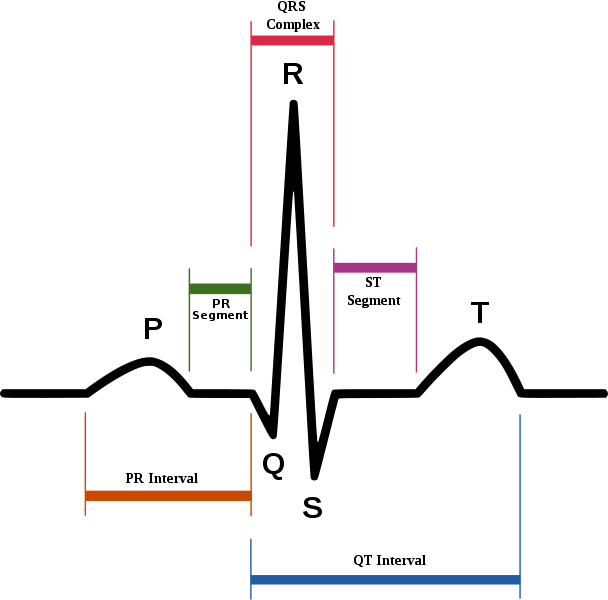
\includegraphics[scale=0.5]{ekg.png}
		\caption{Satu gelombang EKG}
		\label{fig:ecg_signal}
	\end{figure}

Titik fiducial adalah titik-titik yang dapat digunakan sebagai pembanding terjadinya satu siklus atau denyut pada sinyal EKG [xx]. Titik-titik fiducial dalam EKG meliputi titik P,QRS,dan T seperti yang terdapat pada gambar di atas. Titik-titik fiducial ini  merepresentasikan aktivitas listrik dari jantung atrial dan ventrikel. Titik P adalah titik yang menunjukkan aktivitas kontraksi bagian atrial jantung. Segmen PR adalah bentuk sinyal depolarisasi atrial. Selanjutnya qelombang QRS adalah gelombang yang menunjukkan terjadinya kontraksi ventrikel jantung. Terkahir adalah gelombang T yang menunjukkan depolarisasi dari ventrikel.

\section{Premature Ventricular Contractions (PVC)}
Aktivitas denyut jantung yang terjadi pada manusia adalah disebabkan terjadinya aktivitas elektrik jantung yang dilakukan oleh SA-Node dan AV-node\cite{heart_act}. SA-node atau Sino-Atrial Node adalah bagian kecil dari jaringan jantung yang terdapat di bagian atrial dan berfungsi untuk melakukan pelepasan electron yang kemudian akan memacu atrial berkontraksi. Selanjutnya elektron yang dilepaskan oleh SA-node akan ditangkap oleh AV-node melalui jaringan-jaringan kecil di jantung yang kemudian akan dilepaskan kembali oleh AV-node sehingga membuat bagian ventrikel jantung bekontraksi \cite{khandait2012}. Aktifitas-aktifitas pelepasan elektron yang dilakukan oleh SA-node dan AV-node ini lah yang kemudian membuat jantung berdenyut secara ritmik dan teratur. PVC adalah salah satu kelainan jantung yang disebabkan karena ketidaknormalan denyut jantung. Pada PVC, ventrikel berkontraksi secara prematur atau melepaskan elektron sebelum menerima elektron yang dikirimkan oleh SA-node\cite{Kanwar2015}.

\section{Feature Extractions}
\textit{Feature extraction} adalah tahap awal yang dilakukan pada proses deteksi kelainan jantung setelah tahap pre-prosessing pada sinyal EKG. Tahap \textit{feature extraction} ini bertujuan untuk mendapatkan titik P, QRS,T dan nilai-nilai penting lainnya pada gelombang EKG. Nilai-nilai gelombang ini kemudian akan menjadi nilai masukan pada tahap klasifikasi dan dilakukan analisis terhadap nilai-nilai gelombang tersebut. Tingkat akurasi yang dihasilkan pada tahap \textit{feature extraction} cukup menentukan nilai akurasi akhir pada keseluruhan proses deteksi PVC\cite{Huang2015Thesis}. Selain itu \textit{feature extraction} yang baik juga akan membuat proses diagnosa menjadi lebih efisien\cite{Karpagachelvi2010,Chang1987,UMaji}. Karena itu menggunakan algoritma yang sederhana namun tetap mempertahankan akurasi yang optimal dalam tahap \textit{feature extraction} menjadi sangat penting.


\section{Riset Deteksi PVC}
Tahun 1987, Chang\cite{Chang1987} telah mengusulkan sebuah algoritma \textit{feature extraction} yang dapat digunakan secara real-time dan berbasis \textit{microprocessor}. Setelah diujikan kepada 18 orang pasien metode ini mencapai nilai akurasi sebesar 99,3 persen dan sensitivitas 81,12 persen.

Selanjutnya pada tahun 2012, A.Ouelli et al\cite{A.Ouelli2012_AR} menggunakan AR modeling dan algoritma Multi Layer Perceptron untuk membuat metode deteksi arrythmia. Tujuan Ouelli dalam mengajukan metode ini adalah untuk membuktikan bahwa algoritma AR (\textit{Autoregressive} Modeling) memiliki kemampuan untuk menghasilkan hasil \textit{feature extraction} yang sangat baik. Hasil akurasi yang diperoleh Ouelli dengan menggunakan AR modeling dan MLP ini mencapai angka 99,6 persen.

Di tahun yang sama Chen\cite{RobertChen} juga mengusulkan algoritma baru untuk melakukan deteksi PVC secara real-time berbasis Wavelet Transform. Sistem deteksi PVC yang diajukan memiliki dua bagian proses, yaitu proses deteksi puncak R dan proses deteksi sinyal PVC. Algoritma \textit{feature ectraction} yang digunakan adalah algoritma Mallat dan Lipschitz exponent untuk mendapatkan puncak R dan metode \textit{sum of trough} untuk deteksi PVC. Pada saat deteksi PVC digunakan juga RR-interval sebagai nilai threshold. Hasil penelitian ini menghasilkan akurasi sebesar 94,73 persen.

U Maji \cite{UMaji} dalam jurnalnya di tahun 2013 mencoba melakukan metode deteksi AF/Atrial Fibrillation menggunakan Empirical Mode Decomposition dan pendekatan secara statistik. EMD adalah metode dekomposisi sinyal yang telah banyak diterapkan dalam menganalisis morfologi dari sinyal non-stationer seperti ECG. Tahap pertama yang dilakukan adalah melakukan dekomposisi sinyal yang telah dilakukan denoising ke dalam fungsi IMF (Intrinsic Mode Function) kemudian diberikan parameter varian dan standar deviasi untuk melakukan klasifikasi dari setiap data IMF yang ada. Meskipun algoritma EMD ini baru pertama kali diterapka untuk mendeteksi AF, tetapi sudah mampu memiliki nilai \textit{sensitivity} dan \textit{specificity} sebesar 96 persen dan 93 persen. EMD juga termasuk algoritma yang adaptive dan sangat efisien \cite{UMaji}.

Fahruzi \cite{fahruzi} dalam jurnalnya melakukan percobaan deteksi PVC menggunakan kombinas \textit{RR Interval} dan \textit{coeeficient Correlation} untuk mengekstrak informasi penting dari ECG. Pengujian dilakukan dalam rentang waktu data 1 menit yang mewakili bentuk gelombang normal dan gelombang PVC. Percobaan ini menghasilkan akurasi sebesar 99,93 persen dan sensitivitas 97,06 persen. 

Deteksi Arryhthmia juga dilakukan oleh \cite{rameshwari} dengan menggunakan algoritma Pan-Tomkins untuk mendeteksi R peak. \cite{rameshwari} mengatakan bahwa efektifitas deteksi yang dilakukan bergantung dari hasil ekstraksi titik P-Q-R-S dan T yang benar. Pada deteksi PVC yang dilakukan memperoleh sensitivitas sebesar 96,15 persen dan spesifikasi sebesar 92,59 persen.   

\cite{Arief2015} berhasil membuat sistem deteksi PVC pada perangkat Android. Ekstraksi fitur yang dilakukan menggunakan software Android Java eclipse Juno untuk mendapatkan interval RR dan lebar QRS. Kemudian tahap klasifikasi dilakukan dengan algoritma ANN menggunakan software MATLAB. Eksperimen yang dilakukan ini tidak menyebutkan secara jelas algoritma apa yang digunakan dalam ekstraksi fitur. Hasil eksperimen ini memiliki nilai akurasi 96,2 persen, 	spesifikasi 96,58 persen dan sensitivitas 94,58 persen.

Sistem deteksi PVC berbasis mobile lainnya juga dilakukan oleh Pedro\cite{Pedro2014}. Pedro membangun algoritma tersendiri untuk mendeteksi RR interval dan \textit{linear classifier design}. Algoritma ini menghasilkan nilai sensitivitas 90,13 persen dan spesifikasi 82,52 persen.

Huang et al \cite{Huang2015Thesis} pada tahun 2015 juga menggunakan wavelet transform tetapi tanpa menggunakan AR modeling. Dengan classifier yang sama seperti yang dilakukan oleh Zhao yaitu SVM Huang mendapatkan nilai akurasi 93,17 (persen) Melalui thesis miliknya ini akhirnya Huang mengambil kesimpulan bahwa karakteristik gelombang EKG yang dikirimkan kepada classifier sangat menentukan nilai akurasi akhir dari classifier tersebut. 

Lek-Uthai \cite{Lekuthai2014} menggunakan 3 tahap prosedur dalam ektraksi fiturnya yaitu, deteksi QRS complex, \textit{smoothing} untuk mengeliminasi \textit{high frequency} pada gelombang EKG sebelum melakukan ekstraksi bentuk QRS menjadi interval QRS, dan menghilangkan \textit{baseline}. Fitur yang diambil dari gelombang adalah interval RR, bentuk QRS, lebar QRS dan ketinggian ST (ST-level). Hasil dari uji coba ini menghasilkan sensitivitas 99,47 persen dan spesifiksai 99l24 persen. Classifier yang digunakan adalah \textit{binary classification}.

Perbandingan hasil penelitian di atas dapat dilihat pada tabel di bawah ini : 
\begin{figure}[h!]
	\centering
	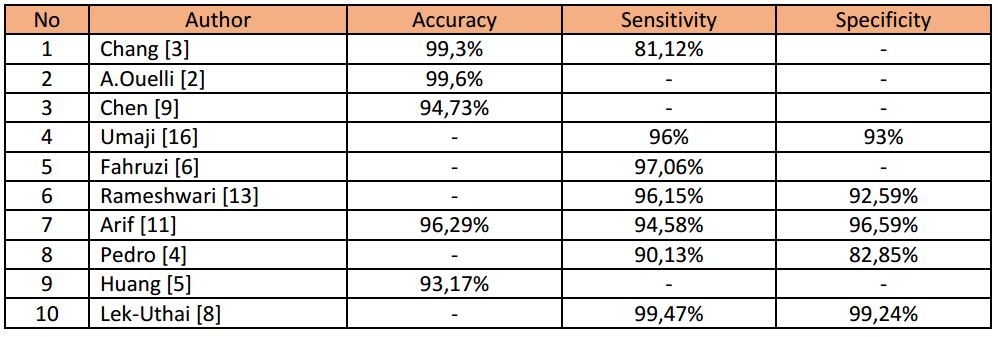
\includegraphics[scale=0.5]{comparison-tab.png}
	\caption{Tabel Perbandingan Hasil Riset}
	\label{fig:my_auth}
\end{figure}

%
\chapter{Metodologi dan Perancangan Sistem}
\section{Metodologi}
\subsection{Riset \textit{Framework}}
	\begin{figure}[h!]
		\centering
		\includegraphics[scale=0.6]{metode-penelitian2.png}
		\caption{Metode Penelitian}
		\label{fig:my_method}
	\end{figure}
	
	Keterangan : 
	\begin{enumerate}
	\item Studi Literatur
	 \subitem Pada tahap ini dilakukan review terhadap penelitian-penelitian yang telah dilakukan sebelumnya. Dilakukan dengan membaca jurnal dan artikel yang berkaitan. Pada tahap ini juga penulis menganalisis masalah dan membuat alasan mengapa masalah tersebut perlu diselesaikan.
	\item Eksperiment Algoritma yang Sudah Ada
	\subitem Melakukan eksperimen terhadap algoritma yang disebutkan dalam literatur yaitu algoritma Empirical Mode Decomposition(EMD).
	\item Analisis Metode
	\subitem Tahap ini adalah tahap analisis metode yang digunakan dalam eksperimen dan bertujuan untuk mengetahui performansi metode tersebut.
	\item Pengembangan Algoritma
	\subitem Tahap ini adalah tahap perumusan dan pengembangan terhadap algoritma EMD yang telah diterapkan sebelumnya.
	\item Uji Algoritma
	\subitem Melakukan pengujian terhadap algoritma yang baru berdasarkan metrik-metrik yang sudah ada
	\item Membandingkan Algoritma
	\subitem Melakukan perbandingan terhadap algoritma yang diusulkan dengan algoritma lain yang menggunakan algoritma klasifikasi sama dan membandingkan algoritma yang dikembangkan dengan algoritma yang sama yang telah dikembangkan pula.
	\item Analisis Hasil
	\subitem Melakukan analisis terhadap hasil uji algoritma yang dikembangkan
	
	\end{enumerate}
\subsection{Data}
Data yang digunakan dalam melakukan penelitian ini adalah sebanyak 48 data elektrokardiogram dari \textit{databse} MIT-BIH, yaitu pada rekaman data ke-100 hingga rekaman data ke-234 \cite{mit-bih}.
	
\subsection{Spesifikasi Perangkat}
Pada penelitian ini digunakan perangkat sebagai berikut :
	\begin{enumerate}
		\item Spesifikasi Perangkat Keras
		\subitem - Laptop Processor Intel(R) Core(TM) i3-2330M @2.20GHz
		\subitem - Memory 4GB 
		\subitem - Hard Drive 250GB
		\item Spesifikasi Perangkat Lunak
		\subitem - Windows 10 Education
		\subitem - Matlab R2015b
 
	\end{enumerate} 

	
\subsection{Metrik}
Metrik yang digunakan dalam melakukan pengukuran algoritma adalah metrik yang juga digunakan pada penelitian-penelitian sebelumnya \cite{Karpagachelvi2010,yasinKaya}. Meliputi akurasi, spesifikasi, dan sensitivitas.

\subparagraph {Persamaan Akurasi}
\begin{equation}\label{akurasi}
%\int_0^1 \frac{f(x)}{g(x)}\ {\rm dx}=\sin x
accuracy = \frac{TP + TN}{TP+FP+FN+TN}
\end{equation}

\subparagraph {Persamaan Spesifikasi}
\begin{equation}\label{spesifikasi}
specificity = \frac{TN}{TN+FP}
\end{equation}

\subparagraph {Persamaan Sensitivitas}
\begin{equation}\label{sensitivitas}
sensitivity = \frac{TP}{TP+FN}
\end{equation}

Di mana TP dan TN melambangkan total dari kebenaran klasifikasi denyut PVC (true positif) dan sebanyak N denyut (true negatif) sampel. Sedangkan FP dan FN melambangkan jumlah dari kesalahan klasifikasi sampel denyut PVC (false positif) dan N denyut (False negative) sampel\cite{yasinKaya}

\subsection{Perbandingan Sistem yang Telah Ada}
Sistem ini akan dibandingkan dengan sistem deteksi PVC lain yang menggunakan \textit{classifier} sama yaitu ANN\cite{Arief2015,Sreelakshmi} dan pada penelitian yang sebelumnya telah menggunakan EMD sebagai \textit{feature extraction} pada deteksi AF\cite{UMaji}.


\section{Rancangan sistem}
\subsection{Arsitektur}
Berikut adalah rancangan sistem yang akan dibuat

	\begin{figure}[h!]
		\centering
		\includegraphics[scale=0.5]{sistem.png}
		\caption{Rancangan Sistem}
		\label{fig:my_sistem}
	\end{figure}

Gambar di atas adalah rancangan umum metode deteksi PVC. Tahap pertama yang dilakukan adalah \textit{pre-processing} ECG yang termasuk di dalamnya adalah \textit{beat parsing, denoising} hingga mendapatkan sinyal yang bersih untuk masuk dalam tahap ekstraksi fitur. Selanjutnya adalah tahap \textit{feature extraction} yang menggunakan algoritma EMD untuk memperoleh bentuk dari gelombang PVC seperti posisi titik R, lebar gelombang QRS dan sebagainya. Berikutnya nilai dari \textit{feature extraction} yang di dapat akan menjadi masukan bagi \textit{classifier} ANN sebagai informasi gelombang PVC yang harus dibaca. Selanjutnya ANN akan membaca semua data gelombang yang masuk dan mendefinisikan gelombang yang termasuk PVC dan yang bukan PVC. Tahap terakhir adalah validasi yang dilakukan untuk memastikan luaran yang didapatkan adalah valid dan sekaligus mengukur nilai akurasi, sensitivitas, dan spesifikasi.
\subsection{Algoritma}	
\begin{figure}[h!]
	\centering
	\includegraphics[scale=0.6]{algo-emd.png}
	\caption{Algoritma EMD\cite{UMaji}}
	\label{fig:emd_algo}
\end{figure}
%
\chapter{Hasil dan Pembahasan}
\section{Hasil Pengujian}
%
\include{Kesimpulan}
%
\cleardoublepage
\addcontentsline{toc}{chapter}{Daftar Pustaka}
\bibliographystyle{acm} %harvard style
\bibliography{References}
%
%\pagebreak
\cleardoublepage
\addcontentsline{toc}{chapter}{Lampiran}
\chapter*{Lampiran}

\end{document}
